\section{Results}
Here we compare the results of our transfer learning algorithm with those of the \textit{REINFORCE} algorithm.
\subsection{CartPole} % (fold)
\label{sub:cartpole}
\subsubsection{Without sparse representation transfer} % (fold)
\label{ssub:cartpole:without_sparse_representation_transfer}
We first explore the differences between learning directly on a target task and first learning on source tasks (i.e. using our transfer learning algorithm), using the metrics that we defined in Section~\ref{sub:tl_metrics}. We consider both 5 and 10 source tasks. The algorithms using 5 source tasks and 10 source tasks are referred to as respectively \textit{TLA 5} and \textit{TLA 10}.
For the regular algorithm, we use the \textit{REINFORCE} that was discussed in Section~\ref{sub:rl_policy_gradient}. The learning curve of both algorithms on the target task is visualized in Figure~\ref{fig:CartPole:reward_target_re-akt5-akt10}.
\begin{figure}[H]
    \centering
    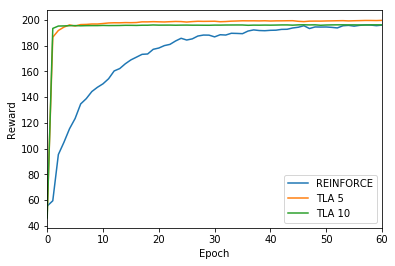
\includegraphics[width=.8\linewidth]{images/results/CartPole/no_sparse_transfer/reward_target_re-akt5-akt10.png}
    \caption[Learning curves for \textit{REINFORCE} and \textit{TLA} for the \emph{CartPole} environment]{Learning curves for the \textit{CartPole} environment of the \textit{REINFORCE} algorithm and our transfer learning algorithm (\textit{TLA}) with 5 source tasks (shown as \textit{TLA 5}) and 10 source tasks (shown as \textit{TLA 10}). The learning curves are only showed until epoch 60 in order to better show the initial performance of the algorithms. All the algorithms were converged and achieved the same rewards after this epoch.}
    \label{fig:CartPole:reward_target_re-akt5-akt10}
\end{figure}
It can be seen visually that, on average, in all the configurations the jumpstart performance is about the same. This is confirmed by using the Wilcoxon signed-rank test. The null-hypothesis is that there is no difference between the jumpstart performance of 2 algorithms. For all the combinations, we get as p-values:
\begin{itemize}
    \item \textit{REINFORCE} and \textit{TLA 5}: $0.413$
    \item \textit{REINFORCE} and \textit{TLA 10}: $0.097$
    \item \textit{TLA 5} and \textit{TLA 10}: $0.415$
\end{itemize}
With a significance level of $0.05$, we can say that the null-hypotheses should be retained and there is no difference between the jumpstart performances of any of the algorithms.\\
However, we can see again in Figure~\ref{fig:CartPole:reward_target_re-akt5-akt10} that \textit{REINFORCE} takes a lot longer on average to reach the maximum reward (which is $200$ in this environment). As a result, the area under curve for \textit{REINFORCE} is $18170.243$ whereas it is $19603.523$ and $19329.318$ for respectively \textit{TLA 5} and \textit{TLA 10}.\\
In every configuration, the maximum reward ($200$) is reached eventually and as such they have the same asymptotic performance.\\

% To further explore the jumpstart performance, we will look at boxplots of the jumpstarts of both algorithms, computed using all the 100 runs of both algorithms. These are shown in Figure~\ref{fig:boxplot_tla_re_5envs}.
% \begin{figure}[H]
%     \centering
%     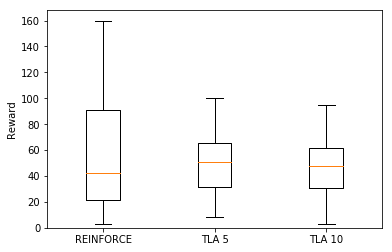
\includegraphics[width=.8\linewidth]{images/results/CartPole/no_sparse_transfer/jumpstart_target_re-akt5-akt10.png}
%     \caption{Boxplot of the jumpstart performance of \textit{REINFORCE} and our transfer learning algorithm (\textit{TLA}).}
%     \label{fig:boxplot_tla_re_5envs}
% \end{figure}
% We can see that, although the mean jumpstart performances are different, there is little difference between the medians: $22.774$ for \textit{REINFORCE} and $23.459$ for our algorithm. However, our algorithm is able to reach a higher initial performance more often. In 75\% of the cases, the jumpstart performance for \textit{REINFORCE} is below $55.535$, while it is $160.595$ for our algorithm.

% subsubsection cartpole:without_sparse_representation_transfer (end)
\subsubsection{With sparse representation transfer} % (fold)
\label{ssub:cartpole:with_sparse_representation_transfer}
\begin{figure}[H]
    \centering
    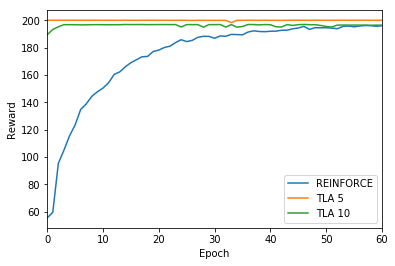
\includegraphics[width=.8\linewidth]{images/results/CartPole/sparse_transfer/reward_target_re-akt5-akt10.png}
    \caption[Learning curves for the \textit{CartPole} environment of \textit{REINFORCE} and \textit{TLA} using sparse representation transfer]{Learning curves for the \emph{CartPole} environment of the \textit{REINFORCE} algorithm and our transfer learning algorithm (\textit{TLA}) with 5 source tasks (shown as \textit{TLA 5}) and 10 source tasks (shown as \textit{TLA 10}). The sparse representation of a randomly chosen source task was transferred to the target task.}
    \label{fig:CartPole:st:reward_target_re-akt5-akt10}
\end{figure}
% subsubsection with_sparse_representation_transfer (end)
% subsection cartpole (end)

\subsection{Acrobot} % (fold)
\label{sub:acrobot}
\subsubsection{Without sparse representation transfer} % (fold)
\label{ssub:acrobot:without_sparse_representation_transfer}
We will start with the same experiment as in Section~\ref{ssub:cartpole:without_sparse_representation_transfer}, but with the \textit{Acrobot} environment.
As can be seen in Figure~\ref{fig:Acrobot:reward_target_re-akt5-akt10}, the average performance of  the \textit{REINFORCE} algorithm on the target task is different from \textit{TLA 5} and \textit{TLA 10}.
\begin{figure}[H]
    \centering
    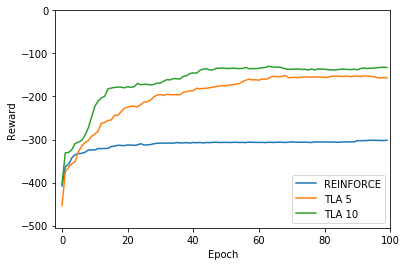
\includegraphics[width=.8\linewidth]{images/results/Acrobot/no_sparse_transfer/reward_target_re-akt5-akt10.png}
    \caption[Learning curves for the \textit{Acrobot} environment of \textit{REINFORCE} and \textit{TLA} for the \emph{Acrobot} environment]{Learning curves of the \textit{REINFORCE} algorithm and our transfer learning algorithm (\textit{TLA}) with 5 source tasks (shown as \textit{TLA 5}) and 10 source tasks (shown as \textit{TLA 10}).}
    \label{fig:Acrobot:reward_target_re-akt5-akt10}
\end{figure}

We will now discuss how exactly the behavior of these algorithms differ.\\
We start by looking at the jumpstart performances. Again, we use the Wilcoxon signed-rank test with the null-hypothesis that there is no difference between the initial performances of the algorithms. As p-values, we get:
\begin{itemize}
    \item \textit{REINFORCE} and \textit{TLA 5}: $0.0047$
    \item \textit{REINFORCE} and \textit{TLA 10}: $0.8143$
    \item \textit{TLA 5} and \textit{TLA 10}: $0.0032$
\end{itemize}
We see that, with a significance level of $0.05$, the jumpstart performance of \textit{TLA 5} is different from the jumpstart performance of the other configurations. To discuss, this further, we look at boxplots of the jumpstart performances of all algorithms, over all their runs. These are shown in Figure~\ref{fig:Acrobot:jumpstart_target_re-akt5-akt10}.
\begin{figure}[htb]
    \centering
    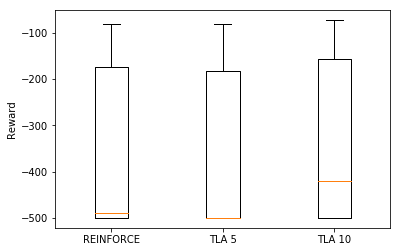
\includegraphics[width=\linewidth]{images/results/Acrobot/no_sparse_transfer/jumpstart_target_re-akt5-akt10.png}
    \caption{Boxplots of the jumpstart performances of \textit{REINFORCE}, \textit{TLA 5} and \textit{TLA 10} using the \textit{Acrobot} environment.}
    \label{fig:Acrobot:jumpstart_target_re-akt5-akt10}
\end{figure}
Indeed, although the medians in all configurations are $-500$ (the lowest reward possible for this environment), the initial performances seem to be spread more for \textit{REINFORCE} and \textit{TLA 10} than for \textit{TLA 5}.\\

As we could already see in Figure~\ref{fig:Acrobot:reward_target_re-akt5-akt10}, the performance of the \textit{REINFORCE} algorithms seems to be lower on average than the other algorithms. This is also visible when looking at the area under curve, which is $-30810.360$ for \textit{REINFORCE} algorithm and $-19437.733$ and $-16223.803$ for respectively \textit{TLA 5} and \textit{TLA 10}.\\

Last, we compare the asymptotic performances, again with the same test and the null-hypotheses that there are no differences between the asymptotic performances. We get the following p-values:
\begin{itemize}
    \item \textit{REINFORCE} and \textit{TLA 5}: $0.0000$
    \item \textit{REINFORCE} and \textit{TLA 10}: $0.0000$
    \item \textit{TLA 5} and \textit{TLA 10}: $0.2902$
\end{itemize}
With a significance level of $0.05$, we can say that there is a difference between \textit{REINFORCE} and \textit{TLA 5} and between \textit{REINFORCE} and \textit{TLA 10}. With the same significance level, we retain the null-hypothesis for \textit{TLA 5} and \textit{TLA 10}. To further discuss these differences, we again look at the boxplots of the asymptotic performances for the three configurations. These are shown in Figure~\ref{fig:Acrobot:asymp_target_re-akt5-akt10}.
\begin{figure}[htb]
    \centering
    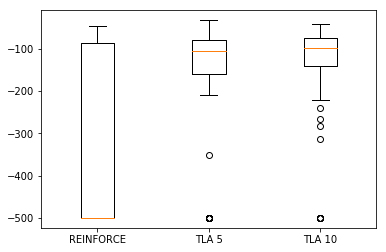
\includegraphics[width=\linewidth]{images/results/Acrobot/no_sparse_transfer/asymp_target_re-akt5-akt10.png}
    \caption{Boxplots of the asymptotic performances of \textit{REINFORCE}, \textit{TLA 5} and \textit{TLA 10} using the \textit{Acrobot} environment.}
    \label{fig:Acrobot:asymp_target_re-akt5-akt10}
\end{figure}
We can see that the median for the \textit{REINFORCE} algorithm is still the lowest possible reward for this environment. The medians of \textit{TLA 5} and \textit{TLA 10} are respectively $-105.3053$ and $-98.3911$. Only some outliers of these algorithms don't get past the minimum reward.

% subsubsection acrobot:without_sparse_representation_transfer (end)
\subsubsection{With sparse representation transfer} % (fold)
\label{ssub:acrobot:with_sparse_representation_transfer}
\begin{figure}[H]
    \centering
    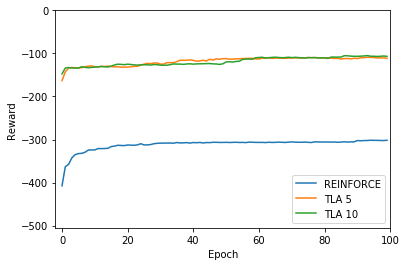
\includegraphics[width=.8\linewidth]{images/results/Acrobot/sparse_transfer/reward_target_re-akt5-akt10.png}
    \caption[Learning curves for the \textit{Acrobot} environment of \textit{REINFORCE} and \textit{TLA} using sparse representation transfer]{Learning curves for the \emph{Acrobot} environment of the \textit{REINFORCE} algorithm and our transfer learning algorithm (\textit{TLA}) with 5 source tasks (shown as \textit{TLA 5}) and 10 source tasks (shown as \textit{TLA 10}). The sparse representation of a randomly chosen source task was transferred to the target task.}
    \label{fig:Acrobot:st:reward_target_re-akt5-akt10}
\end{figure}
% subsubsection acrobot:with_sparse_representation_transfer (end)
\subsubsection{REINFORCE using a source and target task} % (fold)
\label{ssub:reinforce_using_a_source_and_target_task}
\begin{figure}[H]
    \centering
    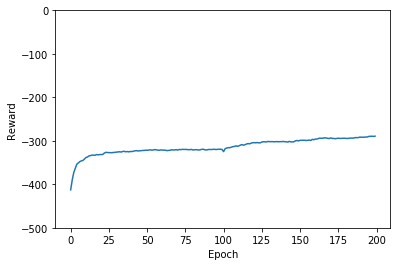
\includegraphics[width=.8\linewidth]{images/results/Acrobot/reinforce_2tasks.png}
    \caption{\textit{REINFORCE} applied for 100 epochs to a randomly chosen source task and afterwards to the target task, using the same network and weight values.}
    \label{fig:Acrobot:reward_reinforce_2tasks}
\end{figure}
% subsubsection reinforce_using_a_source_and_target_task (end)
% subsection acrobot (end)
